\documentclass{article}

\usepackage{amsmath,amssymb,amsfonts,latexsym, amsthm}
\usepackage[spanish,es-noquoting]{babel}
\usepackage[utf8]{inputenc}
\usepackage{xcolor}
\usepackage{empheq}
\usepackage{cancel}
\usepackage{url}
\usepackage[margin=2cm]{geometry}
\usepackage[affil-it]{authblk}
%FONT ===============
%\usepackage{mathptmx}
%\usepackage{cmbright}
\usepackage{ccfonts,eulervm}
\usepackage[T1]{fontenc}
%==================

\newcommand*\widefbox[1]{\fbox{\hspace{2em}#1\hspace{2em}}}
\usepackage{graphicx}
\usepackage{units}
\newtheorem{prop}{Proposición}[section]
\newtheorem{defi}{Definición}[section]
\usepackage{breqn}

\setlength{\parindent}{0pt}

\begin{document}
	
	\title{Potencial Gravitacional de Yukawa en Gravedad $f(R)$}
	\author{Julián Jiménez Cárdenas\thanks{juojimenezca@unal.edu.co}}
	\affil{Universidad Nacional de Colombia.}
	\date{}
	
	\maketitle
	
	\section{Introducción}

Un acercamiento alternativo a la energía oscura es la modificación de la ley de Newton. Tal modificación surge en el límite de campo débil de algunos modelos de gravedad modificada que intentan explicar la materia oscura y la energía oscura como efectos de la curvatura del espacio tiempo. Así, en el límite de campo débil, una modificación de tipo Yukawa de la ley de Newton emerge. Uno de estos modelos es la gravedad-$f(R)$, donde la acción de Hilbert-Einstein, que es lineal respecto al escalar de Ricci $R$, se reemplaza por una función más general de la curvatura, $f(R)$. En el límite de campo débil, el potencial modificado de Newton toma la forma

\begin{equation}\label{yukawaPotential}
\Phi(r)=-\frac{GM}{(1+\delta)r}(1+\delta e^{-r(\lambda)}).
\end{equation}

Donde $M$ es la masa de la fuente puntual, $r$ es la distancia de la partícula de prueba a la fuente, $\delta$ es la fuerza de la corrección de Yukawa y $\lambda$ es la escala a la cual la fuerza de Yukawa actúa (generalmente se identifica esta escala con la longitud de onda del gravitón masivo). Hay una relación entre los parámetros de Yukawa y el Lagrangiano-$f(R)$:

\begin{equation}
	\delta=f_0'-1, \lambda=\sqrt{\frac{-6f_0''}{f_0'}},
\end{equation} 
donde $f_0'=\frac{df(R)}{dR}\Big|_{R=R_0}$ y $f_0'=\frac{d^2f(R)}{dR^2}\Big|_{R=R_0}.$

\section{Acercamiento Newtoniano al problema de dos cuerpos en el potencial de Yukawa}\label{Acercamiento}
En coordenadas polares, $(r,\varphi)$, y con respecto al centro de masa, las ecuaciones del movimiento son
\begin{equation}
\ddot{r}-r\dot{\varphi}^2 = -\nabla \Phi(r),
\end{equation}
\begin{equation}\label{angularConservation}
	\frac{d}{dt}(r^2\dot{\varphi})=0.
\end{equation}

La energía total del sistema se puede escribir como
\begin{equation}
	E_T=\frac{1}{2}\mu(\dot{r}^2+r^2\dot{\varphi}^2)-\frac{GMm}{(1+\delta)r}(1+\delta e^{-r/\lambda}),
\end{equation}

donde $\mu=\frac{Mm}{M+m}$ es la masa reducida. Usando la conservación del momento angular expresada en \eqref{angularConservation}, la energía se puede reescribir de la siguiente manera:

\begin{equation}
	E_T=\frac{1}{2}\mu\dot{r}^2+\underbrace{\frac{L^2}{2\mu r^2}-\frac{GMm}{(1+\delta)}\frac{(1+\delta e^{-r/\lambda})}{r}}_{V_eff(r)}.
\end{equation}

Se define el potencial efectivo como los términos de la energía total que dependen explícitamente de la posición,

\begin{equation}\label{EffPotential}
\boxed{V_{eff}:=\frac{L^2}{2\mu r^2}-\frac{GMm}{(1+\delta)}\frac{(1+\delta e^{-r/\lambda})}{r}.}
\end{equation}

Algunas consideraciones del potencial efectivo son las siguientes:

\begin{itemize}
	\item $\delta\neq -1$, para evitar que el potencial se encuentre indeterminado.
	\item Si $\delta$ toma valores negativos, el segundo término del potencial efectivo permanece atractivo siempre y cuando $\delta > -1$, y el último término se vuelve repulsivo.
	\item La condición $\delta <-1$ hace el segundo término repulsivo, y el tercer término atractivo.
	\item Si $\delta >0$, tanto el segundo como el tercer término son atractivos.
\end{itemize}

\begin{figure}
	\centering
	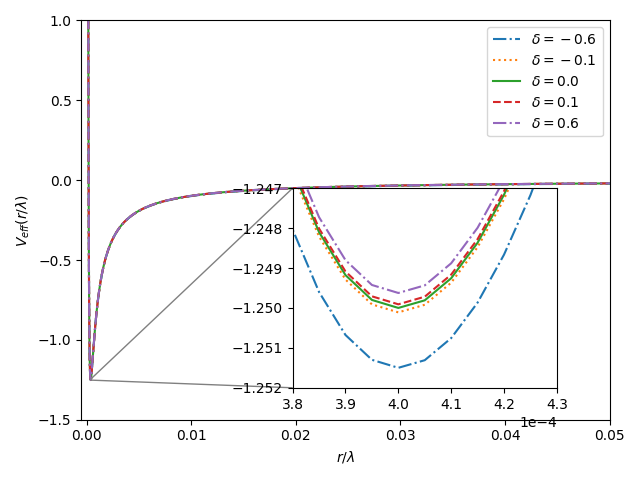
\includegraphics[width=.7\textwidth]{../veff.png}
	\caption{Potencial efectivo en función del cociente $r/\lambda$.}
	\label{fig:effPotential}
\end{figure}

\begin{figure}
	\centering
	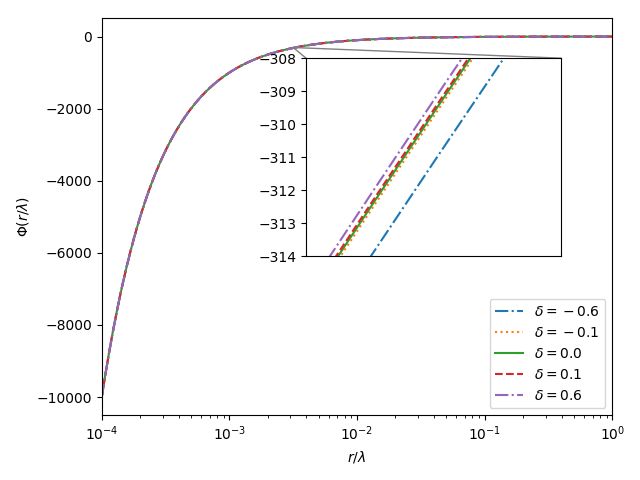
\includegraphics[width=.7\textwidth]{../potential.png}
	\caption{Potencial  en función del cociente $r/\lambda$.}
	\label{fig:potential}
\end{figure}

En las figuras \ref{fig:effPotential} y \ref{fig:potential} se muestra el comportamiento del potencial efectivo y del potencial de Yukawa en función de $r/\lambda$. Se deriva el potencial efectivo respecto a la coordenada radial para determinar los puntos críticos de éste, y encontrar bajó qué condiciones estos puntos críticos son mínimos.

\begin{dmath*}
	\frac{dV_{eff}}{dr}\Big|_{r=r_{crit}}=\frac{-L^2}{\mu r_{crit}^3}+\frac{GMm}{(1+\delta)r_{crit}^2}+\frac{GMm\delta e^{-r_{crit}/\lambda}}{(1+\delta)r_{crit}^2}+\frac{GMm\delta e^{r_{crit}/\lambda}}{\lambda(1+\delta)r_{crit}}=0.
\end{dmath*}
\begin{equation}\label{criticalCondition}
	\implies \frac{L^2}{\mu r_{crit}}=\frac{GMm(\delta e^{-r_{crit}/\lambda}+1)}{(\delta+1)}+\frac{\delta GMme^{-r_{crit}/\lambda}}{\lambda(1+\delta)}r_{crit}.
\end{equation}

Derivando nuevamente el potencial efectivo, se obtiene que

\begin{equation*}
	\frac{d^2V_{eff}}{dr^2}=\frac{3L^2}{\mu r^4}-\frac{2GMm}{(1+\delta)r^3}-\frac{2GMm\delta e^{-r/\lambda}}{(1+\delta)r^3}-\frac{GMm\delta e^{-r/\lambda}}{\lambda(1+\delta)r^2}-\frac{GMm\delta e^{-r/\lambda}}{\lambda(1+\delta)r^2}-\frac{GMm\delta e^{-r/\lambda}}{\lambda^2(1+\delta)r}.
\end{equation*}

De forma más compacta,

\begin{equation}\label{secondForm}
\frac{d^2V_{eff}}{dr^2}=\frac{3L^2}{\mu r^4}- \frac{2GMm}{(1+\delta)r^3}(\delta e^{-r\lambda}+1)-\frac{2GMm\delta e^{-r/\lambda}}{\lambda(1+\delta)r^2}-\frac{GMm\delta e^{-r/\lambda}}{\lambda^2(1+\delta)r}.
\end{equation}

Ahora, resta evaluar la ecuación \eqref{secondForm} en $r=r_{crit}$, y usar la ecuación \eqref{criticalCondition} para reescribir el término del momento angular en función de $r_{crit}$. Así, se encuentra

\begin{dmath*}
	\frac{d^2V_{eff}}{dr^2}\Big|_{r=r_{crit}}=\frac{3GMm(\delta e^{-r_{crit}/\lambda}+1)}{(\delta+1)r_{crit}^3}+\frac{3\delta GMme^{-r_{crit}/\lambda}}{(\delta+1)\lambda r_{crit}^3}r_{crit}-\frac{2GMm}{(1+\delta)r_{crit}^3}(1+\delta e^{-r_{crit}/\lambda})-\frac{2GMm\delta e^{-r_{crit}/\lambda}}{\lambda (1+\delta)r_{crit}^2}-\frac{GMm\delta e^{-r_{crit}/\lambda}}{\lambda^2 (1+\delta)r_{crit}}= \frac{GMm(\delta e^{-r_{crit}/\lambda}+1)}{(\delta+1)r_{crit}^3}+\frac{GMm\delta e^{-r_{crit}/\lambda}}{(1+\delta)r_{crit}^2}-\frac{-GMm\delta e^{-r_{crit}/\lambda}}{\lambda^2(1+\delta)r_{crit}}=\frac{GMme^{-r_{crit}/\lambda}}{(\delta+1)r_{crit}^3}\Big[ \delta\Big(1+\frac{r_{crit}}{\lambda}-\frac{r_{crit}^2}{\lambda^2}\Big)+e^{r/\lambda} \Big].
\end{dmath*}

Para garantizar que este punto crítico sea un mínimo, debe ocurrir que

$$\frac{d^2V_{eff}}{dr^2}\Big|_{r=r_{crit}}>0, \text{ es decir,}$$


$$	\frac{1}{\delta+1}\Big[ \delta\Big(1+\frac{r_{crit}}{\lambda}-\frac{r_{crit}^2}{\lambda^2}\Big)+e^{r/\lambda} \Big]>0.$$

Defina la función $g(x)$, con $x=r_{crit}/\lambda$  como

\begin{equation}\label{minimumFunction}
	\boxed{g(x)\equiv\frac{\delta(1+x-x^2)+e^{x} }{\delta+1}.}
\end{equation}

Cuando se satisfaga que $g(x)>0,$ se tendrá que el punto crítico es un mínimo. Aquí ocurre una de las primeras discrepancias con la referencia \cite{Capozziello}. Capozziello propone que la ecuación que determina si el punto crítico es mínimo es (ver ecuación (12) en \cite{Capozziello})

$$g(x)\equiv\delta(1+x-x^2)+e^{x},$$

sin el cociente de \eqref{minimumFunction}. A pesar de que ambas expresiones difieren sólo por el denominador, éste provoca que los signos de ambas expresiones de $g(x)$ difieran para las mismas condiciones. Por ejemplo, en \cite{Capozziello} se justifica que en el límite $x\rightarrow\infty$, no importa el valor de  $\delta$, $g(x)$ siempre será positivo (la exponencial domina sobre el polinomio multiplicado por $\delta$). En cambio, aunque $x\rightarrow\infty$ en \eqref{minimumFunction}, el signo de ésta dependerá de si $\delta>-1$ o $\delta<-1$. Algunas condiciones en las que \eqref{minimumFunction} es mayor que cero son las siguientes\footnote{Compare las diferencias entre estas condiciones y las condiciones de \cite{Capozziello}.}:

\begin{enumerate}
	\item $\forall\delta\neq-1$ cuando $x\rightarrow 0$.
	\item $\delta>-1$ ó $\delta<-e$ cuando $x\rightarrow 1$.
	\item $\delta>-1$ cuando $x\rightarrow\infty$.
\end{enumerate}

El primer caso, que significa que $r<<\lambda$, es la configuración de un sistema astrofísico cuya dinámica ocurre a escalas mucho menores que la longitud de onda de Compton. En este caso, es válido expandir la exponencial $e^{\pm x}$ es series de Taylor:

\begin{equation}\label{taylorExp}
	e^{\pm x}\approx 1\pm x+\frac{x^2}{2}+O(x^3).
\end{equation}

Reemplazando \eqref{taylorExp} en \eqref{yukawaPotential},

$$\Phi(r)=-\frac{GM}{(1+\delta)r}\Big(1+\delta-\frac{r\delta}{\lambda}+\frac{r^2\delta}{2\lambda^2}+O\Big(\frac{r^3}{\lambda^3}\Big)\Big)=-\frac{GM}{r}+\frac{GM\delta}{\lambda(1+\delta)}+\frac{GM\delta r}{2\lambda^2(1+\delta)}+O\Big(\frac{r^3}{\lambda^3}\Big).$$

Observe que el primer término induce la fuerza Newtoniana usual, el segundo término es un corrimiento constante en la energía que no influye en la dinámica del sistema, y el tercer término genera una aceleración radial constante que se puede escribir como sigue

\begin{equation}\label{pioneer}
	a_{corr}=-\frac{a^*\delta}{2(1+\delta)}\frac{{r^*}^2}{\lambda^2},
\end{equation}

donde $a^*$ es la aceleración Newtoniana de un objeto a una distancia $r^*$. Esta aceleración se suele asociar a la anomalía Pioneer\footnote{Desviación de la aceleración predicha por el modelo Newtoniano, medida por las sondas Pioneer 10 y 11 al alejarse más de 20 unidades astronómicas del sol\cite{anomaly}.}. 

Resulta más sencillo analizar la condición para la existencia del mínimo en el potencial efectivo de Yukawa cuando se hace a órdenes $O(x^2)$ y $O(x^3)$. Es lo que se hará a continuación.

\subsection{Orden $O(x^2)$}
A orden $O(x^2)$, el potencial \eqref{EffPotential} es

\begin{equation}\label{potO2}
	V_{eff}(r)=\frac{L^2}{2\mu r^2}-\frac{GMm}{r}+\frac{\delta GMm}{(1+\delta)\lambda},
\end{equation}


y el mínimo satisface

$$\frac{dV_{eff}}{dr}\Big|_{r_{min}}=-\frac{L^2}{\mu r_{min}^3}+\frac{GMm}{r_{min}^2}=0$$
$$\implies \boxed{r_{min}=\frac{L^2}{\mu GMm}.}$$

Este resultado coincide con el potencial Newtoniano (en \cite{Capozziello} hay un 2 sobrante en el denominador). Sin embargo, el valor del potencial efectivo en el mínimo sí cambia

\begin{equation}\label{order2V}
	V_{eff}(r_{min})=-\frac{1}{2}GMm\Big(\frac{G\mu Mm}{L^2}-\frac{2\delta}{\lambda(1+\delta)}\Big).
\end{equation} 

Observe que en el caso en en el que $\delta=0$, \eqref{order2V} se reduce al potencial efectivo de una órbita circular bajo el potencial Newtoniano.
\subsection{Orden $O(x^3)$}

En este caso, el potencial efectivo \eqref{EffPotential} es
\begin{equation}\label{potO3}
	V_{eff}(r)=\frac{L^2}{2\mu r^2}-\frac{GMm}{r}+\frac{\delta GMm}{(1+\delta)\lambda}-\frac{\delta GMm r}{2(\delta+1)\lambda^2}.
\end{equation}

En este caso, $r_{min}$ es el mismo que a orden $O(x^2)$, debido a que el último término de \eqref{potO3}, que va como $\delta/\lambda^2$, es casi cero. El potencial evaluado en $r_{min}$ es:

\begin{equation}\label{order3V}
	V(r_{min})=-\frac{1}{2}GMm\Big(\frac{G\mu Mm}{L^2}-\frac{2\delta}{(\delta+1)\lambda}\Big)-\frac{L^2\delta}{2(\delta+1)\lambda^2\mu}.
\end{equation}

\section{Ecuaciones de las órbitas}
\subsection{Aproximación de orden $O(x^2)$}

Se usa la conservación del momento angular para escribir
\begin{equation}\label{rdot}
\dot{r}=\dot{\varphi}\frac{dr}{d\varphi}=\frac{L}{\mu r^2}\dfrac{dr}{d\varphi}=-\frac{L}{\mu}\frac{d}{d\varphi}\Big(\frac{1}{r}\Big).
\end{equation}

A segundo orden en la aproximación del término de Yukawa, la energía total del sistema se puede reescribir como

$$E_T=\frac{1}{2}\mu\dot{r}^2+\frac{L^2}{2\mu r^2}-\frac{GMm}{(1+\delta)}\frac{(1+\delta-\delta r/\lambda )}{r}=\frac{1}{2}\mu\Big(-\frac{L}{\mu}\frac{d}{d\varphi}\Big(\frac{1}{r}\Big)\Big)^2+\frac{L^2}{2\mu r^2}-\frac{GMm}{r}+\frac{\delta GMm}{(1+\delta)\lambda},$$

\begin{equation}\label{energyO2}
	\implies E_T=\frac{L^2}{2\mu}\Big(\frac{d}{d\varphi}\Big(\frac{1}{r}\Big)\Big)^2+\frac{L^2}{2\mu r^2}-\frac{GMm}{r}+\frac{\delta GMm}{(1+\delta)\lambda},
\end{equation}
la cual induce la siguiente ecuación diferencial

\begin{equation}\label{diffO2}
	(u')^2+u^2-2\beta_0 u=\beta_1,
\end{equation}

donde $u=1/r$, $u'=\frac{du}{d\varphi}$ y
\begin{gather}\label{constantsO2-I}
		\gamma=GMm,\\
		\beta_0= \frac{\mu\gamma}{L^2} \label{constantsO2-II},\\
		\beta_1=\frac{2\mu E_T}{L^2}-\frac{2\mu\gamma}{L^2\lambda}\frac{\delta}{1+\delta} \label{constantsO2-III}.
\end{gather}

Derivando nuevamente la ecuación \eqref{diffO2}, se obtiene que

\begin{equation}\label{diffO2derived}
	u'(u''+u-\beta_0)=0.
\end{equation}
Ciertamente, como se observó en la sección \ref{Acercamiento}, las desviaciones del potencial de Yukawa son minúsculas comparadas con el caso Newtoniano, lo que provoca que la energía es casi la energía del caso Newtoniano, de modo que se buscarán soluciones Keplerianas (cónicas). Para ello, suponga que

\begin{equation}\label{sol}
	u\equiv\frac{1}{r}=\frac{1+\epsilon\cos\varphi}{\ell}
\end{equation} 

es solución de las ecuaciones diferenciales \eqref{diffO2} y \eqref{diffO2derived}, donde $\ell$ es el \textit{latus rectum} y $\epsilon$ es la excentricidad. Insertando \eqref{sol} en \eqref{diffO2derived},

$$\frac{-\epsilon\sin\varphi}{\ell}\Big(\cancel{\frac{-\epsilon\cos\varphi}{\ell}}+\frac{1}{\ell}(1+\cancel{\epsilon\cos\varphi})-\beta_0\Big)=0,$$

\begin{equation}\label{latusO2}
	\boxed{\ell=\frac{1}{\beta_0}.}
\end{equation}

Ahora, sustituyendo \eqref{sol} en \eqref{diffO2}:
$$\frac{\epsilon^2\sin^2\varphi}{\ell^2}+\frac{1+\cancel{2\epsilon\cos\varphi}+\epsilon^2\cos^2\varphi}{\ell^2}-\frac{2}{\ell^2}(1+\cancel{\epsilon\cos\varphi})=\beta_1,$$

$$\implies \frac{\epsilon^2}{\ell^2}+\frac{1}{\ell^2}-\frac{2}{\ell^2}=\beta_1,$$

\begin{equation}\label{eccentricityO2}
	\boxed{\epsilon^2=1+\ell^2\beta_1=1+\frac{\beta_1}{\beta_0^2}.}
\end{equation}
\begin{figure}
	\centering
	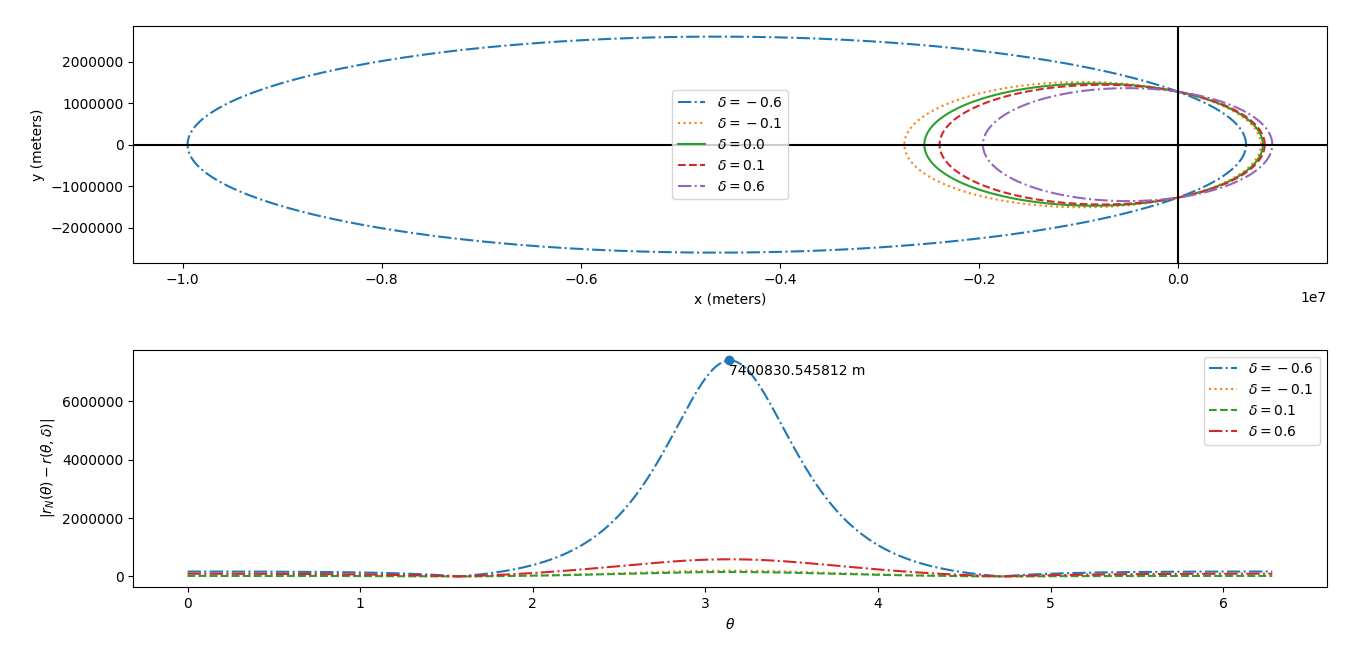
\includegraphics[width=.8\textwidth]{../orbits2.png}
	\caption{De arriba a abajo: órbitas obtenidas para la aproximación a orden $O(x^2)$ para algunos valores de $\delta$. Diferencia absoluta de la distancia en función del ángulo para estas órbitas y la respectiva órbita Newtoniana (con las mismas constantes del movimiento).}
	\label{fig:orbitas2}
\end{figure}
La excentricidad escrita en términos de las constantes del movimiento es
\begin{equation}
	\epsilon^2=1-\frac{2L^2}{\mu\gamma}\frac{\delta}{(1+\delta)\lambda}+\frac{2E_TL^2\mu}{\mu^2\gamma^2},
\end{equation}

que, para $\delta=0$ se reduce al valor Newtoniano:

\begin{equation}
	\epsilon^2=1+\frac{2E_TL^2}{\mu\gamma^2}.
\end{equation}

\subsection{Aproximación de orden $O(x^3)$}

A tercer orden, la ecuación diferencial \eqref{diffO2} adquiere un nuevo término

\begin{equation}\label{diffO3}
	(u')^2+u^2-2\beta_0 u-\beta_2\frac{1}{u}=\beta_1,
\end{equation}

donde $\beta_0$ y $\beta_1$ están dados por \eqref{constantsO2-II} y \eqref{constantsO2-III}, respectivamente; y
\begin{equation}\label{constantbeta2}
	\beta_2=\frac{\mu\gamma\delta}{L^2\lambda^2(1+\delta)}.
\end{equation}

Aquí nos encontramos con uno de los errores más graves de \cite{Capozziello}. La definición proveída por \cite{Capozziello} es $$\beta_2=\frac{\mu \gamma \delta}{2 L^{2} \lambda(1+\delta)},$$ cuyas unidades (distancia$^{-2}$) son claramente distintas a las de \eqref{constantbeta2} (distancia$^{-3}$). A largo plazo ésto tendrá consecuencias en las unidades de la excentricidad de \cite{Capozziello}. Tomando la derivada de la ecuación \eqref{diffO3}:

\begin{equation}\label{diffO3derived}
	u'\Big(u''+u+\frac{\beta_2}{2u^2}-\beta_0\Big)=0.
\end{equation}

De nuevo, bajo la suposición de que las solución \eqref{sol} funciona en este caso, se introduce en \eqref{diffO3derived} para hallar el \textit{latus rectum}.
$$\frac{-\epsilon\cos\varphi}{\ell}+\frac{1}{\ell}(1+\epsilon\cos\varphi)+\frac{\beta_2\ell^2}{2(1+\epsilon\cos\varphi)^2}-\beta_0=0.$$

Evaluando esta última expresión en $\varphi=0, \pi$, se obtienen las expresiones

\begin{gather}
	\epsilon^2(1-\beta_0\ell)+2\epsilon(1-\ell\beta_0)-\ell\beta_0+\frac{\beta_2\ell^3}{2}+1=0 \text{ y }\label{sum1}\\
	\epsilon^2(1-\beta_0\ell)-2\epsilon(1-\ell\beta_0)-\ell\beta_0+\frac{\beta_2\ell^3}{2}+1=0\label{sum2}.
\end{gather}

Restando \eqref{sum1}-\eqref{sum2}, 
\begin{figure}
	\centering
	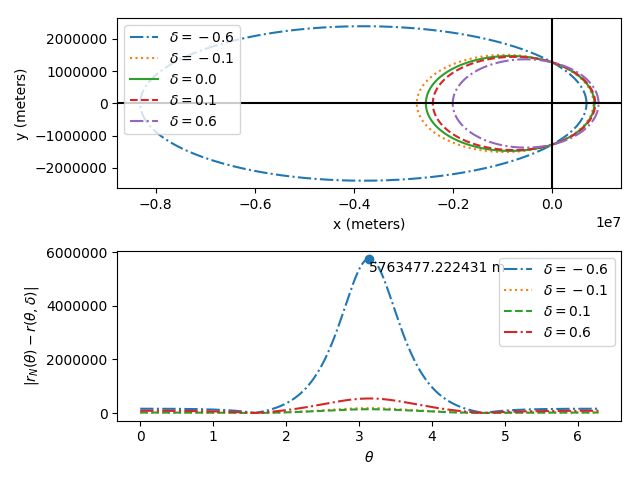
\includegraphics[width=.7\textwidth]{../orbits3.png}
	\caption{De arriba a abajo: órbitas obtenidas para la aproximación a orden $O(x^3)$ para algunos valores de $\delta$. Diferencia absoluta de la distancia en función del ángulo para estas órbitas y la respectiva órbita Newtoniana (con las mismas constantes del movimiento).}
	\label{fig:orbitas3}
\end{figure}

$$4\epsilon(1-\beta_0\ell)=0,$$

lo que implica que $\ell=\beta_0^{-1}$, y el \textit{latus rectum} no varía entre los órdenes $O(x^2)$ y $O(x^3).$ Ahora, introduciendo \eqref{sol} en \eqref{diffO3derived},

$$\Big(-\frac{\epsilon\sin\varphi}{\ell}\Big)^2+\frac{(1+\epsilon\cos\varphi)^2}{\ell^2}+\frac{-2-2\epsilon\cos\varphi}{\ell^2}-\frac{\beta_2\ell}{1+\epsilon\cos\varphi}=\beta_1,$$

$$\implies \frac{\epsilon^2\sin^2\varphi+\epsilon^2\cos^2\varphi+\cancel{2\epsilon\cos\varphi}+1-2-\cancel{2\epsilon\cos\varphi}}{\ell^2}-\frac{\beta_2\ell}{1+\epsilon\cos\varphi}=\beta_1,$$

$$\implies \frac{\epsilon^2-1}{\ell^2}-\frac{\beta_2\ell}{1+\epsilon\cos\varphi}=\beta_1,$$

\begin{equation}\label{epsEqO3}
	(\epsilon^2-1)(1+\epsilon\cos\varphi)-\beta_2\ell^3=\beta_1\ell^2(1+\epsilon\cos\varphi).
\end{equation}
Evaluando \eqref{epsEqO3} en $\varphi=0,\pi$ se obtiene, respectivamente
\begin{gather}
	\epsilon^3+\epsilon^2-1-\epsilon-\beta_2\ell^3-\beta_1\ell^2(1+\epsilon)=0\label{oneEps},\\
	-\epsilon^3+\epsilon^2-1+\epsilon-\beta_2\ell^3-\beta_1\ell^2(1-\epsilon)=0\label{twoEps}.
\end{gather}

Sumando \eqref{oneEps}+\eqref{twoEps}, se determina el valor de $\epsilon$:
\begin{equation}\label{eccO3}
	\boxed{\epsilon^2=1+\beta_2\ell^3+\beta_1\ell^2=1+\frac{\beta_2}{\beta_0^3}+\frac{\beta_1}{\beta_0^2}.}
\end{equation}

Observe que la excentricidad \eqref{eccO3} es efectivamente adimensional y satisface el límite a orden $O(x^2)$, es decir, si $\beta_{2}=0$, se obtiene \eqref{eccentricityO2}. En cambio, la excentricidad propuesta por \cite{Capozziello} es

$$\epsilon^2=1+\ell^{2} \beta_{1}-4 \beta_{2},$$

y no es coherente dimensionalmente hablando, dado que, como se comentó anteriormente, las unidades de $\beta_{2}$ son de distancia$^{-2}$ según \cite{Capozziello}, y el último término no sería adimensional. En términos de las constantes del movimiento, la excentricidad \eqref{eccO3} es

\begin{equation}
	\epsilon^2=1+\frac{2L^2E_T}{\mu\gamma^2}-\frac{2L^2}{\mu\gamma}\frac{\delta}{(1+\delta)\lambda}+\frac{\delta L^4}{\lambda^2(1+\delta)\mu^2\gamma^2}.
\end{equation}

\section{Precesión en el potencial de Yukawa}
Para calcular analíticamente el corrimiento en el periastro debido al término del potencial de Yukawa, se estudian pequeñas perturbaciones de las órbitas cerrada. Para ello, se reescribe la energía total como

\begin{equation}\label{preEnergy}
	(u')^2+u^2+\frac{g(u)}{L^2}=\frac{2\mu E_T}{L^2}-\frac{2\mu\gamma}{L^2\lambda}\frac{\delta}{1+\delta},
\end{equation}

donde $g(u)$ representa la interacción gravitacional. Se impone una órbita cerrada definida por una distancia mínima y máxima al centro (foco)

\begin{gather*}
	r_-|_{\varphi=0}=a(1-\epsilon),\\
	r_+|_{\varphi=\pi}=a(1+\epsilon),
\end{gather*}

respectivamente. $a$ es el semieje mayor de la órbita. Estos valores corresponden a $u_0=1/r_-$ y $u_1=1/r_+$. Dado que $u'|_{u=u_0}=u'|_{u=u_1}=0$ (dado que son mínimo y máximo de la función), la ecuación \eqref{preEnergy} induce las dos siguientes condiciones:

\begin{gather}
	u_{0}^{2}+\frac{g\left(u_{0}\right)}{L^{2}}=\frac{2 \mu E_{T}}{L^{2}}-\frac{2 \mu \gamma}{L^{2} \lambda} \frac{\delta}{1+\delta},\label{con1}\\
	u_{1}^{2}+\frac{g\left(u_{1}\right)}{L^{2}}=\frac{2 \mu E_{T}}{L^{2}}-\frac{2 \mu \gamma}{L^{2} \lambda} \frac{\delta}{1+\delta}\label{con2},
\end{gather}

de las cuales se obtienen ligaduras para el momento angular y la energía total:
\begin{gather}
	L^{2}=\frac{g\left(u_{0}\right)-g\left(u_{1}\right)}{u_{1}^{2}-u_{0}^{2}}\label{Lpre}\\
	E_{T}=\frac{u_{1}^{2} g\left(u_{0}\right)-u_{0}^{2} g\left(u_{1}\right)}{2 \mu\left(u_{1}^{2}-u_{0}^{2}\right)}+\frac{ \gamma \delta}{(1+\delta) \lambda}\label{ETpre}.
\end{gather}
La ecuación \eqref{Lpre} se obtuvo restando \eqref{con1}-\eqref{con2}; la ecuación \eqref{ETpre} se obtuvo sumando \eqref{con1}+\eqref{con2}, usando \eqref{Lpre} y despejando $E_T$. Escribiendo el momento angular y la energía en términos de $u_0$ y $u_1$, se puede despejar $u'$ de la ecuación diferencial \eqref{preEnergy}, de modo que dependa de $(u_0,u_1,u),$ es decir, \eqref{preEnergy} se transforma en

\begin{equation}\label{simplified}
	u'=\sqrt{G(u_0,u_1,u)},
\end{equation}

donde $G(u_0,u_1,u)$ es\footnote{Aquí \cite{Capozziello} tiene un error de digitación: aparece una $b$ que no tiene nada que ver.}

\begin{equation}
	G\left(u_{0}, u_{1}, u\right)=\frac{g\left(u_{0}\right)\left(u_{1}^{2}-u^{2}\right)+g\left(u_{1}\right)\left(u^{2}-u_{0}^{2}\right)-\left(u_1^{2}-u_{0}^{2}\right) g(u)}{g\left(u_{0}\right)-g\left(u_{1}\right)}.
\end{equation}

Se puede encontrar el ángulo requerido para moverse desde $r_-$ hasta $r_+$ integrando la ecuación \eqref{simplified}:

\begin{equation}\label{integralPrecession}
	\varphi(r_+)-\varphi(r_-)=\int_{u_0}^{u_1} G(u_0,u_1,u)^{-1/2}du.
\end{equation}

En el caso de que no hubiese precesión, la partícula iría de $r_-$ a $r_+$ y volvería si el ángulo $\varphi$ aumenta $2\pi$. Ésto implica que $r(\varphi)$ sería periódica, con período $2\pi$. Si hay precesión, $r(\varphi)$ deja de ser periódica, y es posible determinar la precesión como la medida de qué tanto se corre la posición del perihelio (o afelio) por cada revolución:

\begin{equation}\label{precession}
	\omega=2|\varphi(r_+)-\varphi(r_-)|-2\pi.
\end{equation}

Cuando se aproxima la exponencial del potencial de Yukawa a orden $O(x^2)$, la función $g(u)$ se compone únicamente del potencial Newtoniano,

\begin{equation}
	g(u)=-2\mu\gamma u=2\mu\Phi_N(1/u),
\end{equation}

donde $\Phi_N(1/u)$ es el potencial clásico de Newton. Así, a este orden la precesión no existe, como se espera del potencial Newtoniano. Sin embargo, cuando se aproxima el término exponencial a orden $O(x^3)$, se obtiene que la función $g(u)$ es

\begin{equation}\label{gO3}
	g(u)=2\mu\Phi_N(1/u)-\frac{\mu\gamma\delta}{\lambda^2(1+\delta)}\frac{1}{u}.
\end{equation}

Nuevamente, \cite{Capozziello} omite un $\lambda$ en el denominador, proponiendo la expresión
$$g(u)=2 \mu \Phi_{N}(1 / u)-\frac{\mu \gamma \delta}{\lambda(1+\delta)} \frac{1}{u},$$

sin coherencia dimensional. La diferencia entre esta ecuación y \eqref{gO3} impide que se obtengan los mismos resultados que los de \cite{Capozziello}. Para resolver numéricamente la ecuación \eqref{integralPrecession}, se hacen los cambios de variables:

\begin{gather*}
	u_1=u_0+\eta,\\
	u=u_0+\eta v,
\end{gather*}
con $0<v<1$. Así, \eqref{integralPrecession} se reescribe como
\begin{equation}
	\Delta\varphi\equiv\varphi(r_+)-\varphi(r_-)=\eta\int_{0}^{1}h(u_0, u_0+\eta,\lambda,\delta, u_0+\eta v)dv,
\end{equation}
donde
\begin{equation}
	h(u_0, u_0+\eta,\lambda,\delta, u_0+\eta v)=\frac{1}{\sqrt{G(u_0,u_0+\eta,\lambda,\delta,u_0+\eta v)}}.
\end{equation}
\begin{thebibliography}{9}
	\bibitem{Capozziello} S. Capozziello, M. De Laurentis, Annalen der Physik 524, 545 (2012) 
	
	\bibitem{Lee} K. Lee, F. A. Jenet, R. H. Price, N. Wex, M. Kramer Astrophys.
	
	\bibitem{Capozziello2} S. Capozziello, M. De Laurentis, Phys. Rept. 509, 167 (2011).
	J. 722, 1589-1597 (2010)
	
	\bibitem{main} I. Martino, R. Lazkoz. Analysis of the Yukawa gravitational potential in f (R) gravity I: semiclassical periastron advance.
	
	\bibitem{anomaly} Referencia sobre la anomalía Pioneer: \url{https://en.wikipedia.org/wiki/Pioneer_anomaly}
\end{thebibliography}
\end{document}